\section{Visual Fidelity Guaranteed Sampling Approach}\label{sec:sol}
Due to the hardness of the Problem~\ref{prob:def}, we first introduce a straight-forward solution (i.e., uniform random sampling) for it in Section~\ref{sec:random}.
Then, we propose a visual fidelity guaranteed sampling approach in Section~\ref{sec:greedy}.
Last, we devise several optimizations to improve the efficiency and effectiveness of our proposal in Section~\ref{sec:opt}.


\subsection{Uniform Random Sampling Algorithm}\label{sec:random}
The straight forward solution for Problem~\ref{prob:def} is uniform random sampling $\rand$.
As the pseudocode in Algorithm~\ref{alg:rand} shown, it selects $k$ trajectories from $\D$ randomly, which stores in $\oR$,
then render these selected trajectories in $\oR$ as the visualization result.

\begin{algorithm}
    \caption{$\rand(\D,k=\alpha |\D|)$} \label{alg:rand}
    \begin{algorithmic}[1]
    \State Initialize result set $\oR \leftarrow \emptyset$
    \While{$|\oR| < k$}
        \State $tmp \leftarrow \mathsf{RandomSampling(\D-\oR)}$
        \State $\oR \leftarrow \oR \cup \{ tmp \}$
    \EndWhile
    \State Return $\oR$
    \end{algorithmic}

\end{algorithm}



Obviously, the uniform random sampling algorithm has good performance.
However, it does not provide any guarantee on the visual fidelity of the sampled result set.


%Trajectory data $\D$\cite{xxx} consists of almost 10K trajectories which collected by Didi company.
%The visualization result of the whole dataset $\D$ is illustrated in Figure~\ref{fig:demo}(b).
%Figure~\ref{fig:demo}(b) shows the visualization result of uniform random sampling result of $\D$ with $k=100$.
%The difference between the visualization results in Figures~\ref{fig:demo}(a) and (b) are obvious from user's perspective.

%\begin{figure}
% \centering
% \small
% \begin{tabular}{cc}
%   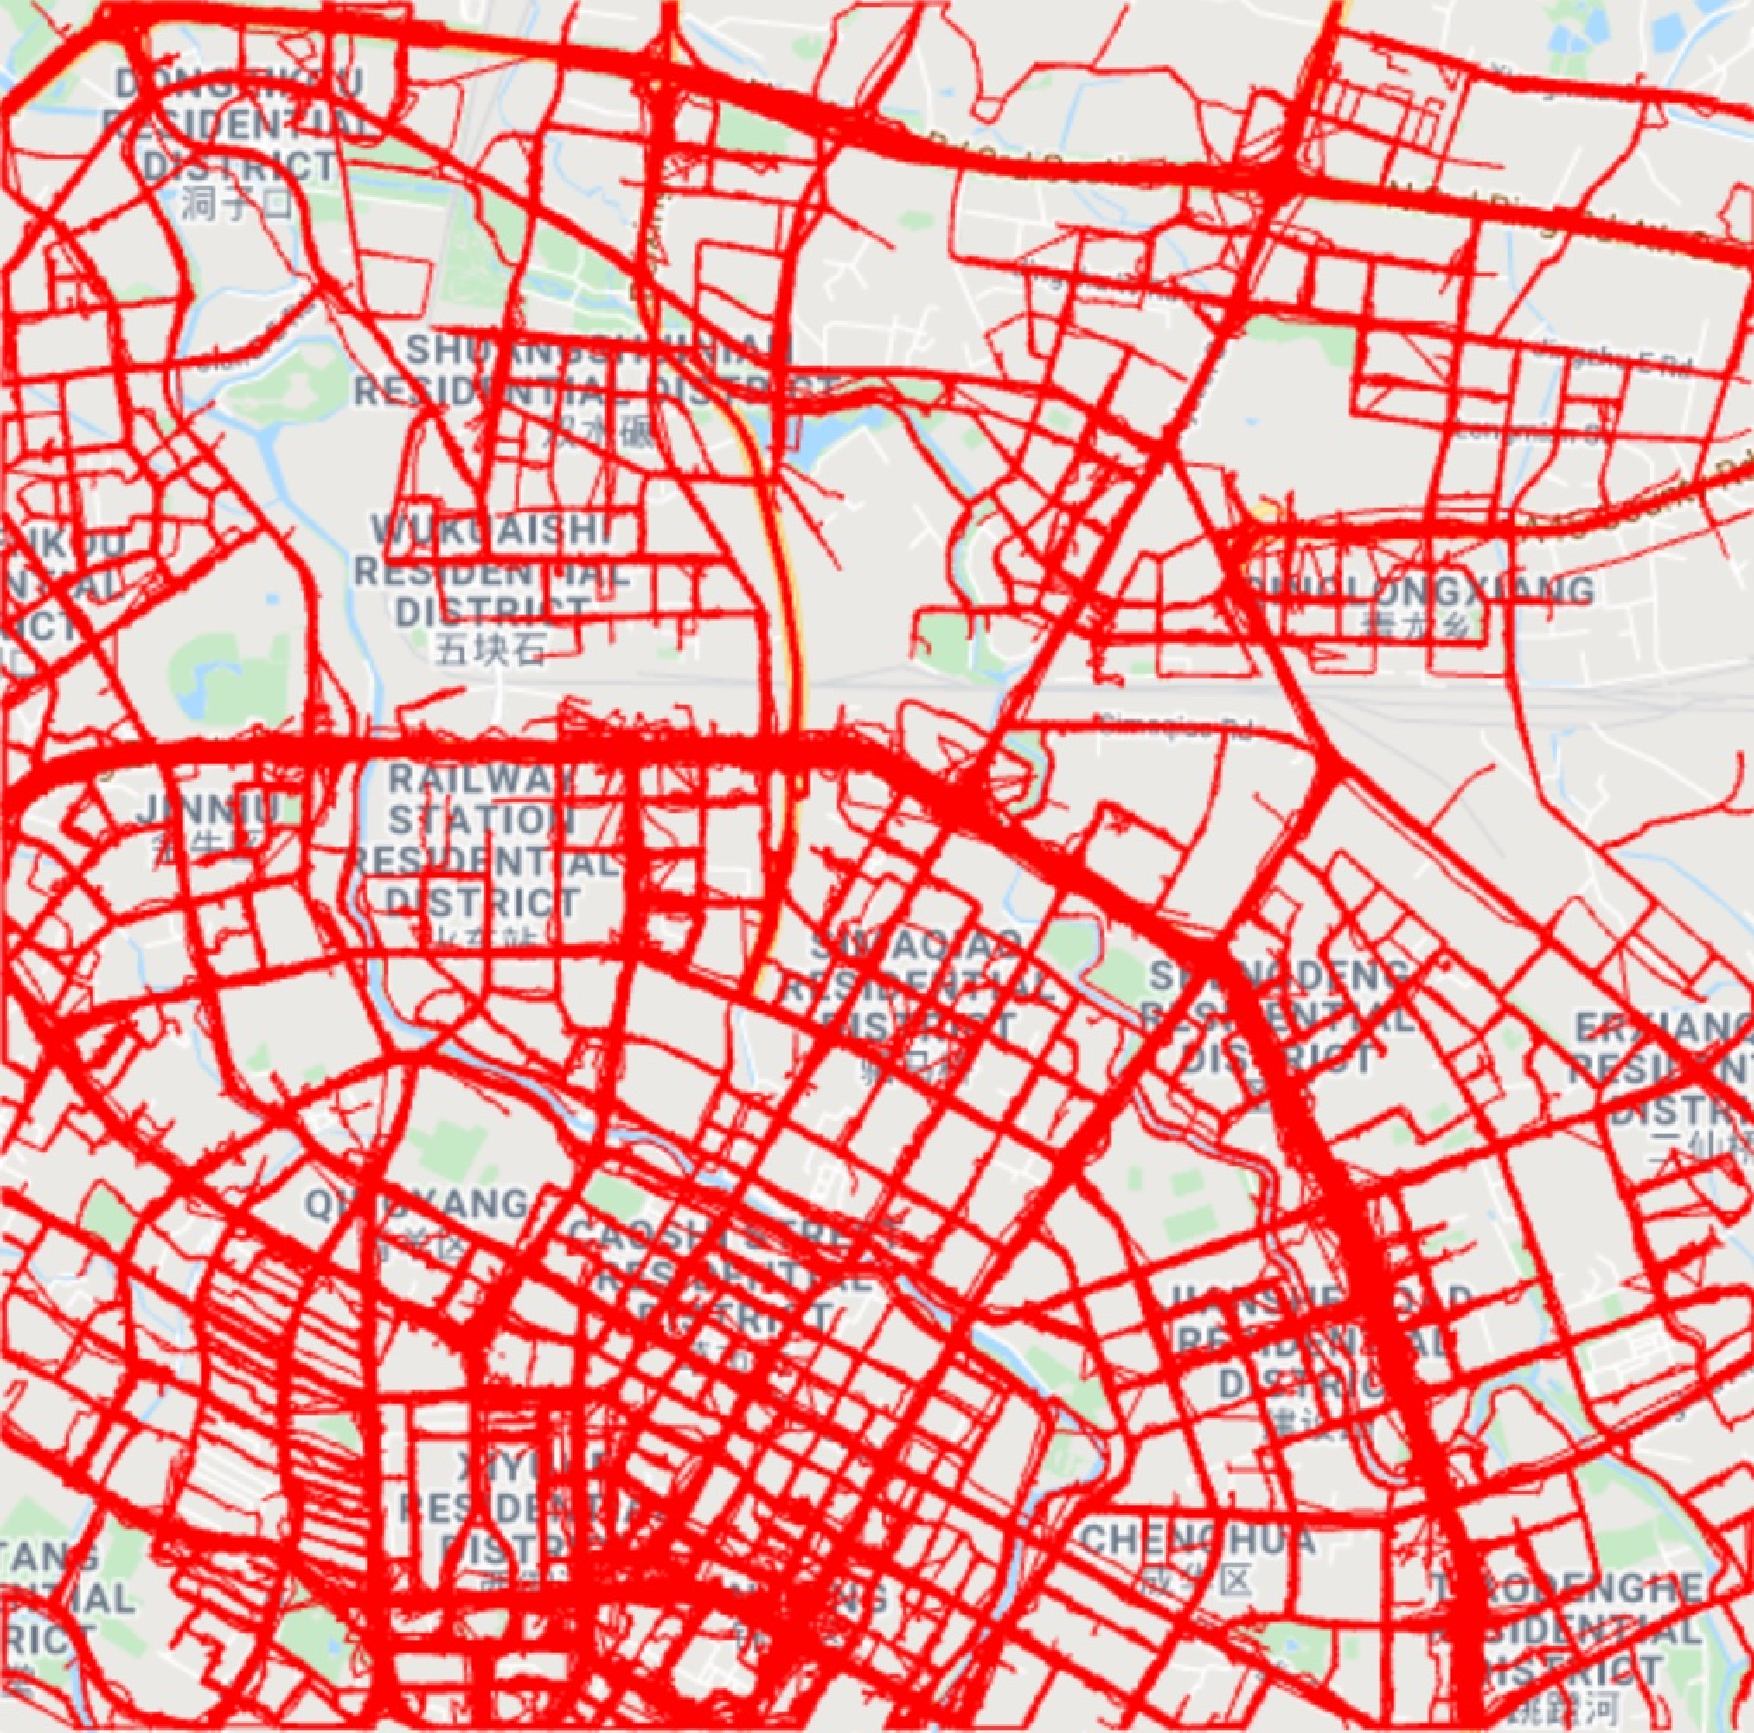
\includegraphics[width=0.45\columnwidth]{chengdu_total}
%   &
%   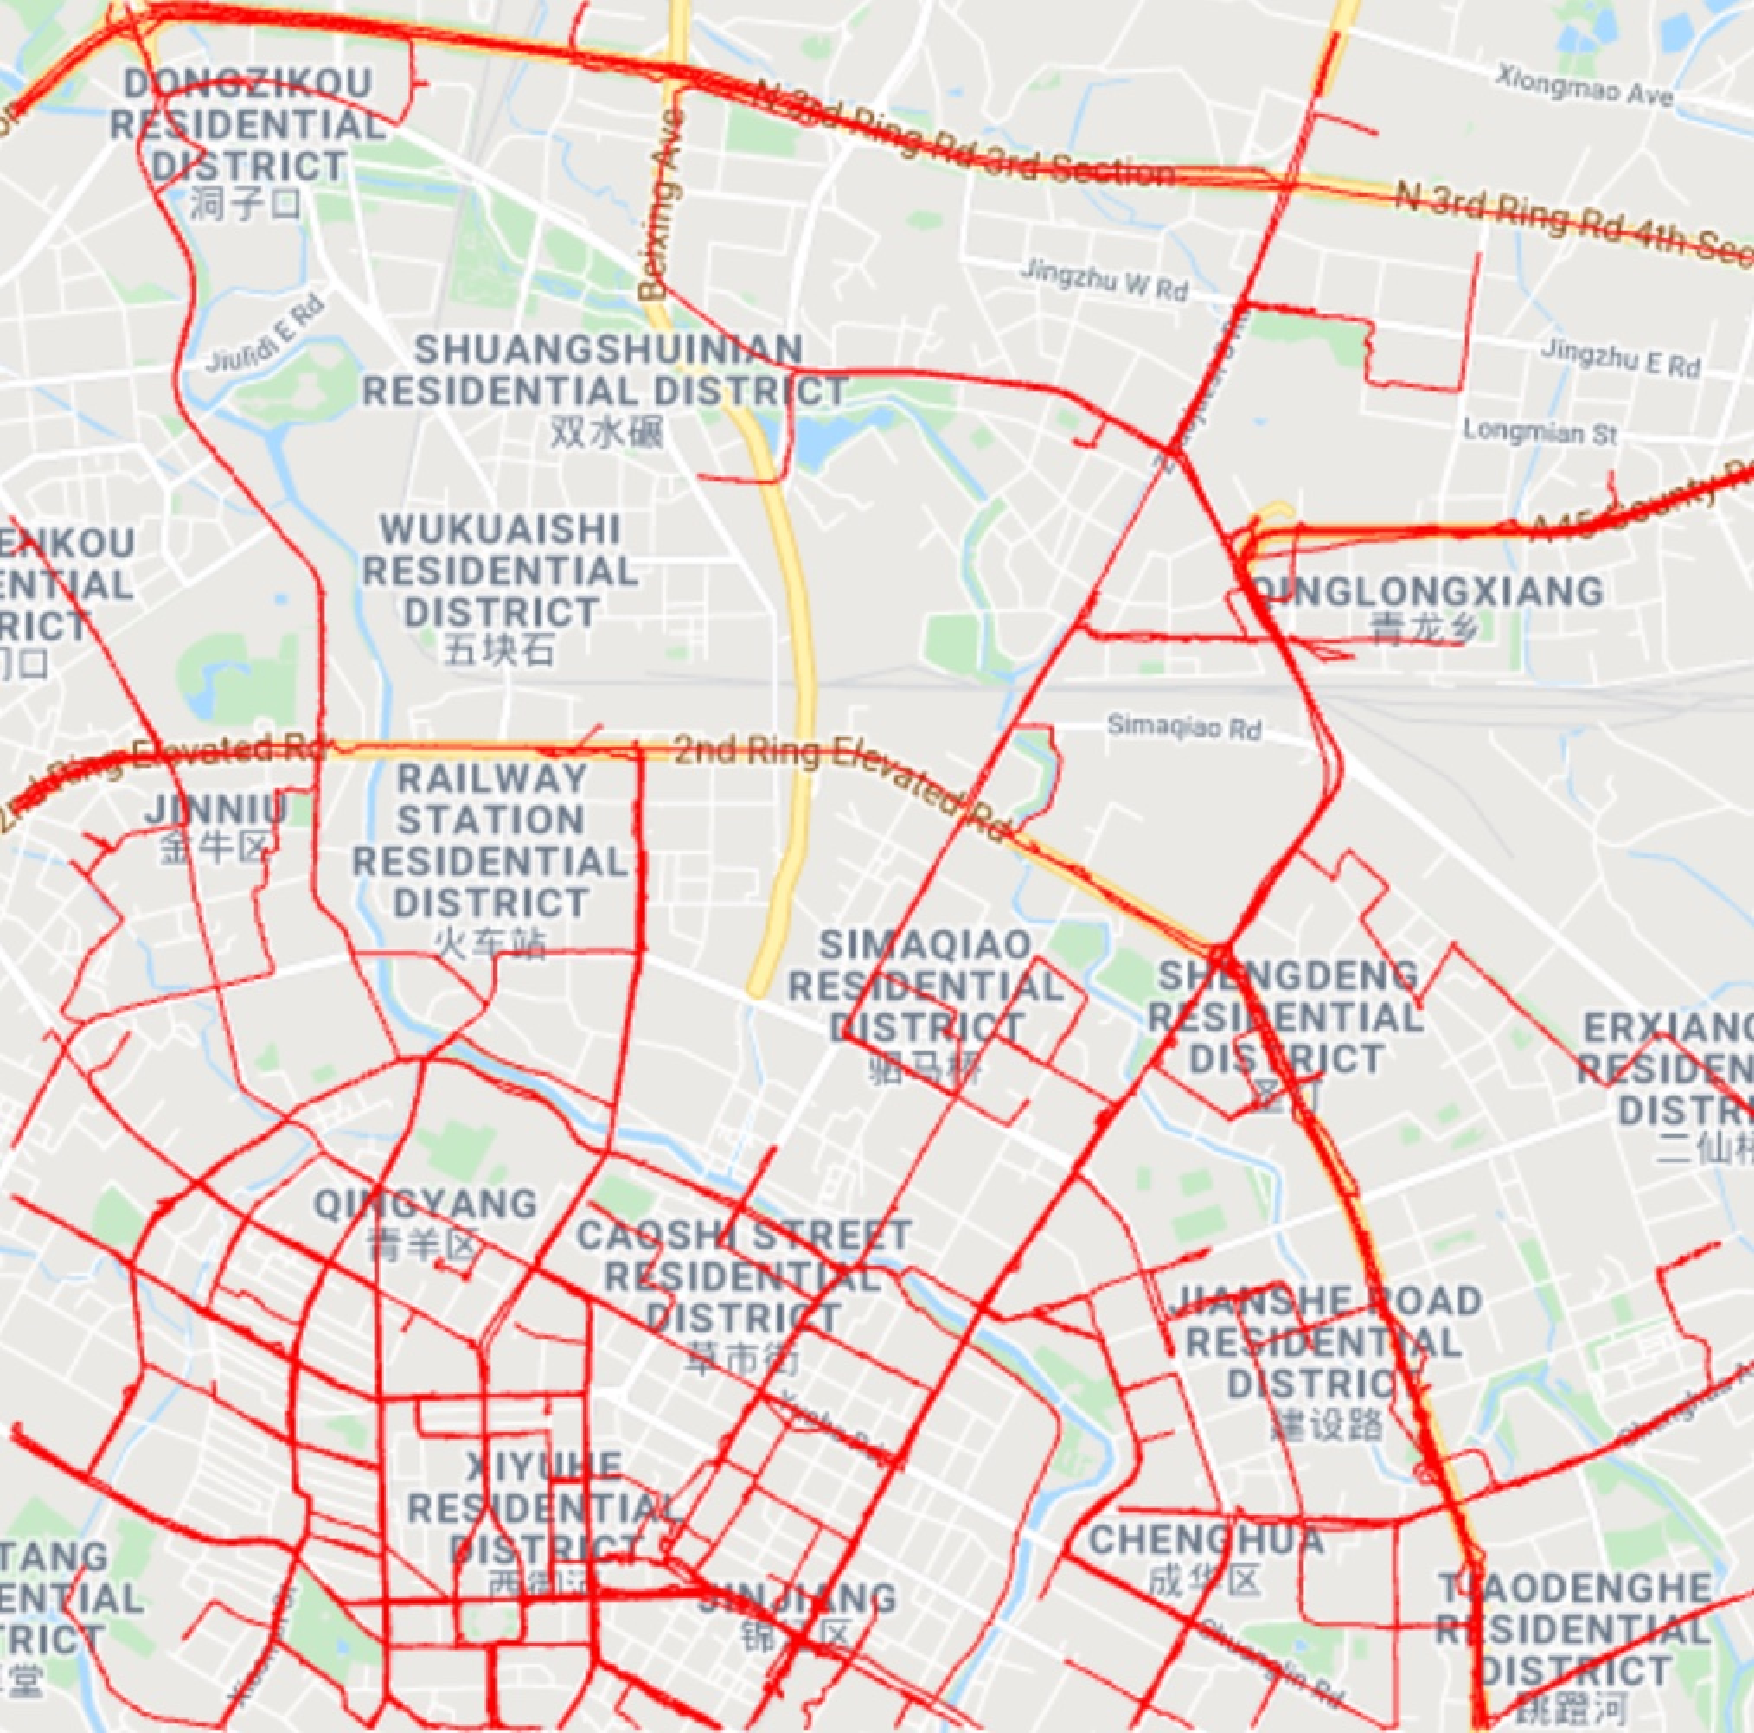
\includegraphics[width=0.45\columnwidth]{chengdu_sampling}
%   \\
%   (a) Dataset $\D$
%   &
%   (b) Uniform sampling $\oR$
% \end{tabular}
% \caption{Visualization results of trajectory set in Chengdu}
% \label{fig:demo}
%\end{figure}

\subsection{Visual Fidelity Guaranteed Sampling Algorithm}\label{sec:greedy}
In this section, we present our visual fidelity guaranteed sampling algorithm for Problem~\ref{prob:def}.
We start our presentation by elaborating the correlation between visual fidelity of sampled set $\oR$ and user zoom level.
For a given sampled set $\oR \subseteq \D$, it has different visual fidelity loss values at different user zoom levels.
The reason is the resolutions of $\oR$'s visualized result are different at different zoom levels.
%The reason is the pixel size will be updated at different zoom level.
%\QM{The reason is the map are of the same canvas region will be updated at different zoom level.}
For example, Google map~\cite{googlemap} provides zoom levels range from 0 to 20,
where level 0 is the lowest level (e.g., the whole world), level 20 is the highest level (e.g., individual building, if available).
In order to devise a zoom level oblivious visualization for sampled dataset $\oR$,
we use the highest zoom level to define the size of each pixel in the canvas in our problem.
It means for each trajectory $t_i \in \D$, it is a set of pixels in the canvas at the highest zoom level.

The visual fidelity guaranteed sampling algorithm employs greedy paradigm.
In particular, it finds the trajectory $tmp$ in $\D$ which maximize the result set of $|\oR \cup tmp|$ at each iteration, as Line~\ref{line:max} shown in Algorithm~\ref{alg:greedy}.
It terminates after $k=\alpha |\D|$ iterations and returns $\oR$ as result set for rendering.

\vspace{-2mm}
\begin{algorithm}
    \caption{$\vats(\D,k=\alpha |\D|)$} \label{alg:greedy}
    \begin{algorithmic}[1]
    \State Initialize result set $\oR \leftarrow \emptyset$
    \While{$|\oR| < k$}
        \State $tmp \leftarrow argmax_{t_i \in \D} |\oR \cup t_i|$ \label{line:max}
        \State $\oR \leftarrow \oR \cup \{ tmp \}$
    \EndWhile
    \State Return $\oR$
    \end{algorithmic}
\end{algorithm}
\vspace{-2mm}

Interestingly, Algorithm~\ref{alg:greedy} offers theoretical visual fidelity guarantee of the returning result $\oR$, as proved in Theorem~\ref{the:ratio}.

\begin{theorem}~\label{the:ratio}
Algorithm~\ref{alg:greedy} provides $1-(1-1/k)^k \geq (1-1/e) \approx 0.632$ approximation result for large-scale trajectory visualization problem (i.e., Problem~\ref{prob:def}).
\end{theorem}

\begin{proof}
The optimal solution of Problem~\ref{prob:def} covers $OPT$ pixels in $k$ iterations.
Let $a_i$ be the number of newly covered pixels at the $i$-th iteration, $b_i$ is the total number of covered pixels up to the $i$-th iteration (i.e., $b_i = \sum_{j=1}^{i}a_i$),
and $c_i$ be the uncovered pixels after $i$-th iteration (i.e., $c_i = OPT-b_i$).
According to greedy paradigm, we can conclude the number of newly covered pixels at the $(i+1)$-th iteration is always greater than or equal to $\frac{1}{k}$ of the number of uncovered pixels after the $i$-th iteration, i.e., $a_{i+1} \geq \frac{c_i}{k}$.
We prove Theorem~\ref{the:ratio} by proving $c_{i+1} \leq (1-1/k)^{i+1} \cdot OPT$.
It holds $c_1 \leq (1-1/k) \cdot OPT$ as follows.
\begin{align} \nonumber
& a_1 \geq c_0 \cdot 1/k = 1/k \cdot OPT \text{~~~as we concluded~~~} a_{i+1} \geq \frac{c_i}{k}\\ \nonumber
 \Leftrightarrow  & b_1 \geq 1/k \cdot OPT  \Leftrightarrow  -b_1 \leq - 1/k \cdot OPT  \text{~~~as~~~} a_1 = b_1\\ \nonumber
 \Leftrightarrow & OPT - b_ 1 \leq OPT - 1/k \cdot OPT  \Leftrightarrow  c_1 \leq (1-1/k) \cdot OPT
\end{align}
For inductive hypothesis assume $c_{i} \leq (1-1/k)^i \cdot OPT$. Thus,
\begin{align} \nonumber
& c_{i+1} = c_i - a_{i+1} \leq c_i - c_i/k = (1-1/k) \cdot c_i = (1-1/k)^{i+1} \cdot OPT
\end{align}

Hence, it holds $c_k \leq (1-1/k)^{k} \cdot OPT$.
It is equivalent to $b_k \geq (1 - (1-1/k)^{k}) \cdot OPT \geq (1-1/e) \cdot OPT \approx 0.632 \cdot OPT$.
\end{proof}


\subsection{Optimization Techniques}\label{sec:opt}
With the above analysis, Algorithm~\ref{alg:greedy} ($\vats$) provides a visual fidelity guaranteed sampling algorithm for large-scale trajectory data visualization problem.
However, it is inefficient for (very) large trajectory dataset (e.g., millions of trajectories) as the time complexity analyzed in the following Lemma~\ref{lem:cost}.

\begin{lemma}[Time Complexity]~\label{lem:cost}
Given trajectory dataset $\D$ and an integer $k = \alpha |\D|$, the time complexity of Algorithm~\ref{alg:greedy} is $O(\alpha \cdot m \cdot |\D|^2)$, where $m$ is the maximum length of all trajectories in dataset $\D$.
\end{lemma}

\begin{proof}
At each iteration ($k = \alpha |\D|$ iterations in total),
it computes the uncovered pixels of each trajectory in dataset $\D$ with $O(m)$ cost.
The dataset $\D$ has $O(|D|)$ trajectories.
Thus, the total cost is $O(k \cdot m \cdot |\D|)=O(\alpha \cdot m \cdot |\D|^2)$.
\end{proof}

\stitle{Example} Given \pt{} trajectory dataset, it has 2.39 millions of taxi trajectories, the maximum length in it is 3,490.
It takes 413.6 seconds to return a subset $\oR$ with sampling rate $0.1\%$.
Obviously, it is impractical for interactive trajectory explorations.

Due to the inefficient of our visual fidelity guaranteed sampling approach in Algorithm~\ref{alg:greedy},
we then devise performance optimizations to accelerate its running time.
The core idea is utilizing the submodularity of the covered pixels of result set $\oR$, as shown in Lemma~\ref{lem:submodular}.

\begin{lemma}[Submodularity]\label{lem:submodular}
Suppose the contribution of trajectory $t$ to the result set $\oR$ is $\Delta(\oR, t) = |\oR \cup t| - |\oR|$.
Given a trajectory $t$ and two result sets $\oR,\oR^{'}$, where $\oR \subset \oR^{'}$ and $t \notin \oR$,
it holds $ \Delta(\oR, t) \geq \Delta(\oR^{'}, t)$.
\end{lemma}

\begin{proof}
The contribution value of trajectory $t$ to a given result set $\oR$ (e.g., $\Delta(\oR, t) = |\oR \cup t| - |\oR|$) is the new covered pixels of $t$ w.r.t. result set $\oR$, i.e., $|t| - |\oR \cap t|$.
It holds $t \cap \oR \subseteq  t \cap \oR^{'}$ as $\oR^{'}$ is a superset of $\oR$.
Thus, we have $|t| - |t \cap \oR| \geq |t| - |t \cap \oR^{'}|$.
Hence, it holds $\Delta(\oR, t) = |\oR \cup t| - |\oR| \geq |\oR^{'} \cup t| - |\oR^{'}|= \Delta(\oR^{'}, t)$.
\end{proof}

\begin{figure}
 \centering
 \small
 \begin{tabular}{cc}
   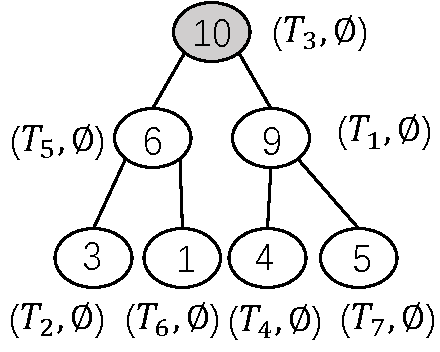
\includegraphics[width=0.35\columnwidth]{1st}
   &
   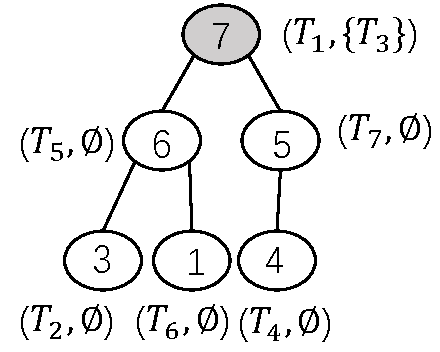
\includegraphics[width=0.35\columnwidth]{2nd}
   \\
   (A) 1st iteration
   &
   (B) 2nd iteration
 \end{tabular}
 \vspace{-3mm}
 \caption{An illustration of lazy computing manner via Lemma~\ref{lem:submodular}} \label{fig:heap}
 \vspace{-6mm}
\end{figure}


With the help of submodularity in Lemma~\ref{lem:submodular}, it reduces many unnecessary trajectory contribution value computations.
In particular, we maintains a max-heap for the number of uncovered pixels of each trajectory,
we employ lazy computing manner, i.e., only compute the contributions of a given trajectory when it is necessary.
Fig.~\ref{fig:heap}(a) shows a tiny max-heap example about the numbers of uncovered pixels of each trajectory from $t_1$ to $t_7$ with result set $\oR=\emptyset$.
At the 1st iteration, the root node of the max-heap will be selected, i.e., $t_3$ in Fig.~\ref{fig:heap}(A).
At the 2nd iteration, the number of uncovered pixels of the root node $t_1$ is updated to 7 w.r.t. result set $\oR = \{t_3 \}$ (see gray node at Fig.~\ref{fig:heap}(B)).
Then $t_1$ will be selected at the 2nd iteration without computing the number of uncovered pixels in other trajectories, i.e., all white nodes at Fig.~\ref{fig:heap}(B).
The reason is their contributions will be less than 7 via the submodularity shown in Lemma~\ref{lem:submodular}.

%In summary, the number of uncovered pixels in each trajectory will only be computed with the latest result set $\oR$ when it is necessary in the lazy computing manner,
%e.g., only $t_1$ will be updated at the 2nd iteration in Figure~\ref{fig:heap}.
%It reduces many unnecessary computations through the lazy updating manner, e.g., all white nodes did not update at the 2nd iteration in the above example.

%We then analyze the time complexity of Algorithm~\ref{alg:greedy} with lazy computing manner in Theorem~\ref{lem:lazy}.
%
%\begin{lemma}[Optimized Time Complexity]~\label{lem:lazy}
%Given trajectory dataset $\D$ and an integer $k= \alpha |\D|$, the time complexity of Algorithm~\ref{alg:greedy} with lazy computing manner is $O(\alpha \cdot m \cdot x |\D| \log |\D|)$, where $x$ is the number of contribution computations among all $k$ iterations and $x \ll |\D|$.
%\end{lemma}
%
%\begin{proof}
%It first takes $O(|\D|)$ time to construct the max-heap~\cite{cormen2009introduction}.
%It incurs $O( m \cdot x \log |\D|)$ cost to select the trajectory with maximum uncovered pixels at each iteration ($k$ iterations in total).
%Hence, the overall cost is $O(|\D| + k \cdot m \cdot t \log |\D|)$.
%\end{proof}
The performance of Algorithm~\ref{alg:greedy} is improved significantly as we only compute its contribution values when it is necessary.
To exemplify, Algorithm~\ref{alg:greedy} costs 413.6 seconds to return the results with sampling rate $0.1\%$ \pt{} taxi trajectory dataset.
However, it only needs 1.2 seconds in our performance optimized $\vats$.



\begin{figure}[t]
	\centering
	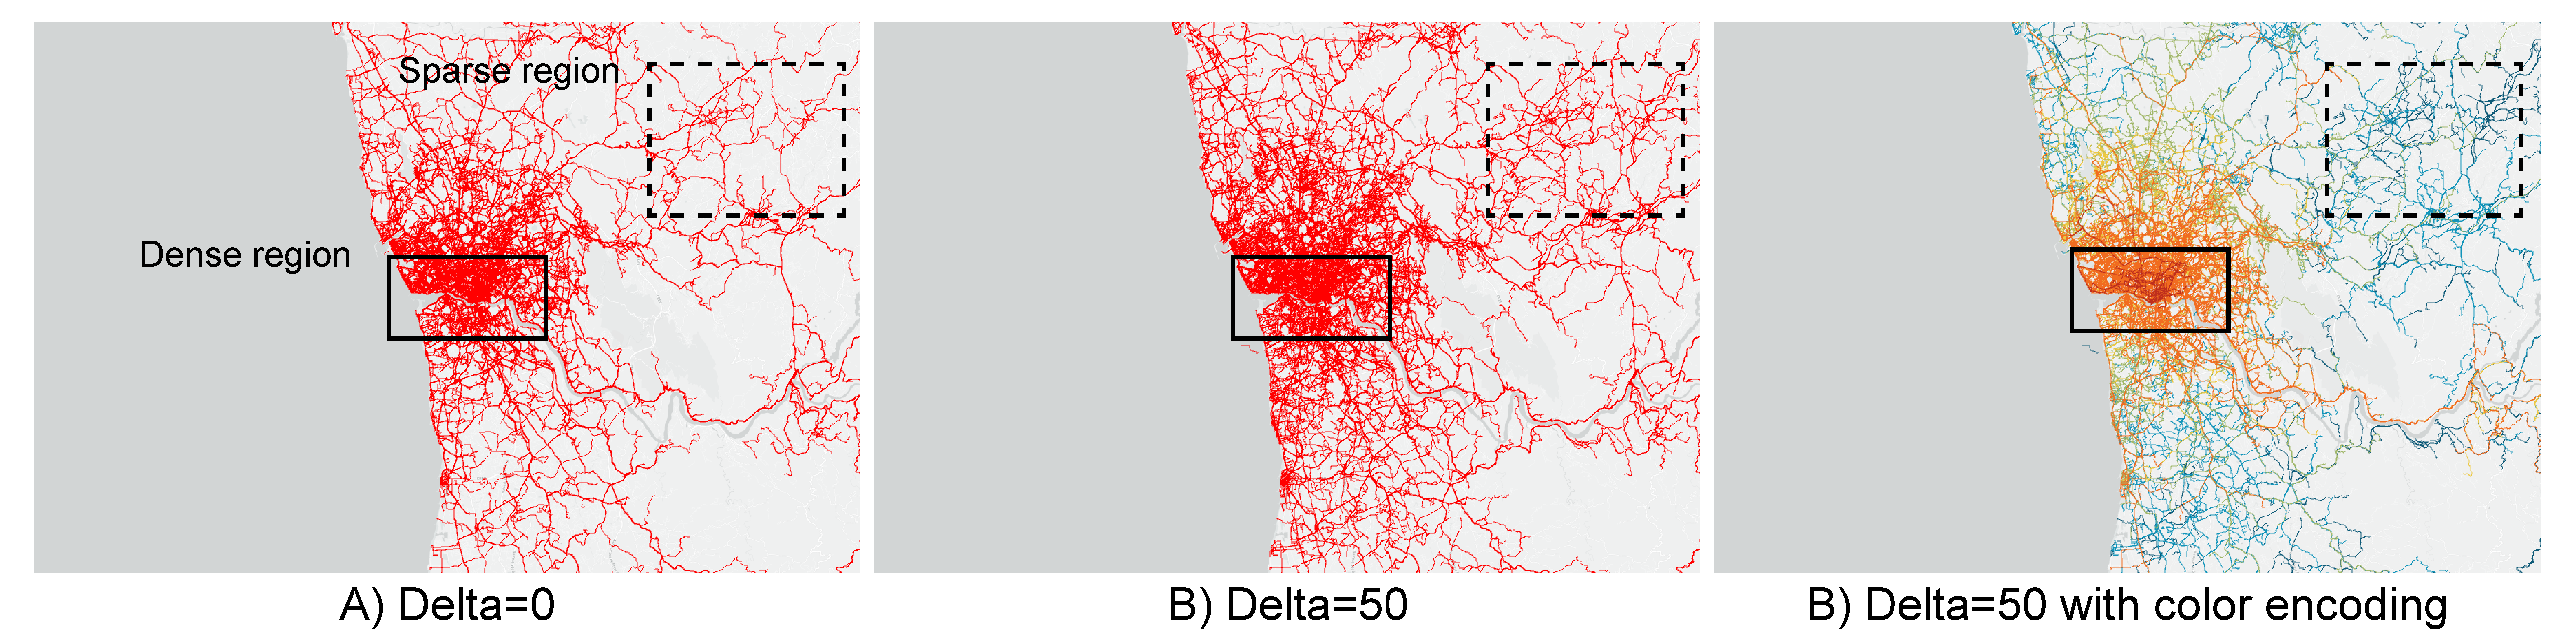
\includegraphics[width=0.48\textwidth]{pictures/problemsolveing/delta_motivation.pdf}
	\vspace{-3mm}
	\caption{Advance Approach $\avats$ with \pt{} trajectory dataset, sampling rate is $0.5\%$: (A) $\vats{}$, (B) $\avats$, and (C) $\cavats$}
	\label{fig:delta}
	 \vspace{-3mm}
\end{figure}


%https://developers.google.com/maps/documentation/maps-static/dev-guide#Zoomlevels

%\begin{figure}[t]
%	\centering
%	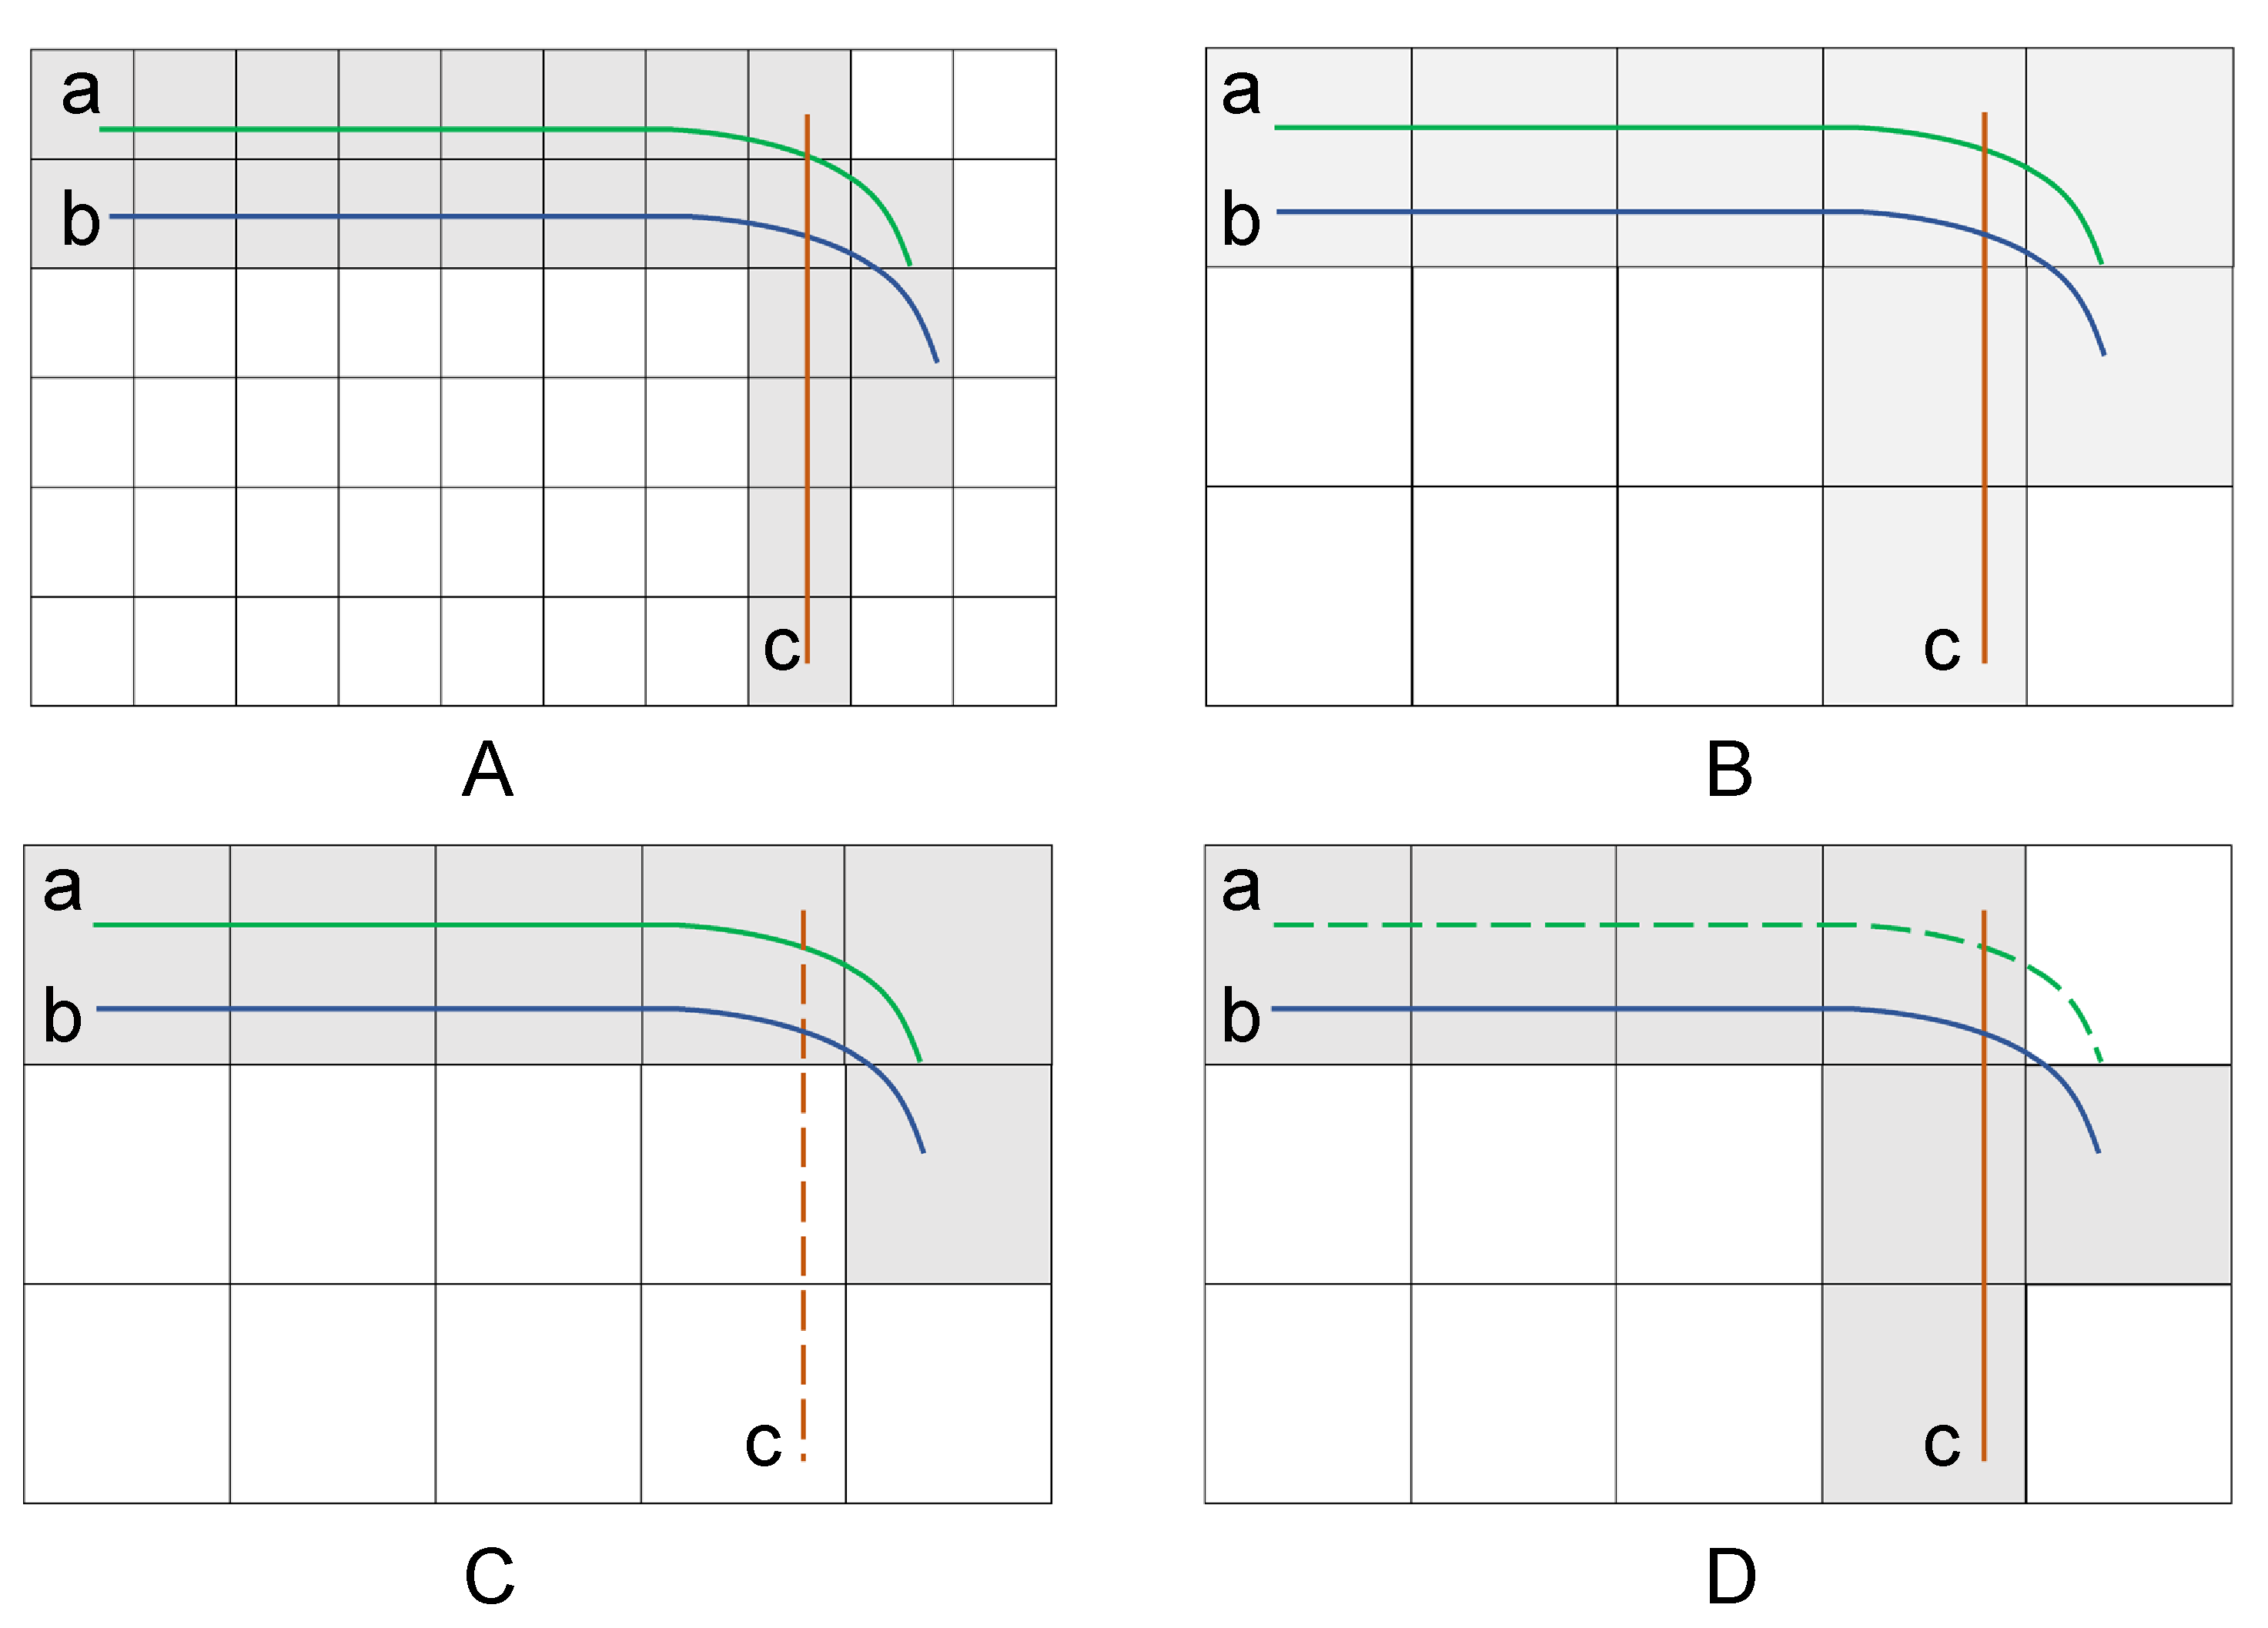
\includegraphics[width=0.4\textwidth]{pictures/problemsolveing/one_to_many.pdf}
%	\vspace{-5mm}
%	\caption{Resolution inconsistency}
%	\vspace{-5mm}
%	\label{fig:one_to_many}
%\end{figure}

%\subsection{One-to-many strategy}~\label{sec:one_to_many}
%Since we detect the covered pixels in the highest level, two trajectories may be very close to each other but share very few pixels, which will lead to more information loss in the low zoom view as figure~\ref{fig:one_to_many}.
%We next elaborate a ``one-to-many'' strategy to further optimize the visual quality of our proposed technique.
%Recalling we use the highest zoom level to define the pixel size in the canvas.
%Thus, our visual quality guaranteed sampling algorithm is zoom-level oblivious, e.g., it guarantees the visual quality of result set $\oR$ at every zoom level.
%However, users always do not use/need the highest zoom level in visualization applications.
%For example, Google map shows city and streets at zoom level 1 and 15, respectively~\footnote{\url{https://developers.google.com/maps/documentation/}}.
%Motivated by the above observation, we devise ``one-to-many'' strategy by introducing a visual tolerance parameter $\delta$ to optimize the visual quality for users.
%Specifically, suppose the pixel with location $(x,y)$ in canvas is covered by result set $\oR$,
%the ``one-to-many'' strategy will ignore all the pixels around $(x,y)$ within $\delta$ offset distance, i.e., all pixels from $(x-\delta, y-\delta)$ to $(x+\delta, y+\delta)$ will be skipped.
%We will demonstrate the effectiveness of the visual tolerance $\delta$ in experimental evaluations.
%
%%https://developers.google.com/maps/documentation/maps-static/dev-guide#Zoomlevels
%\begin{figure}[t]
%	\centering
%	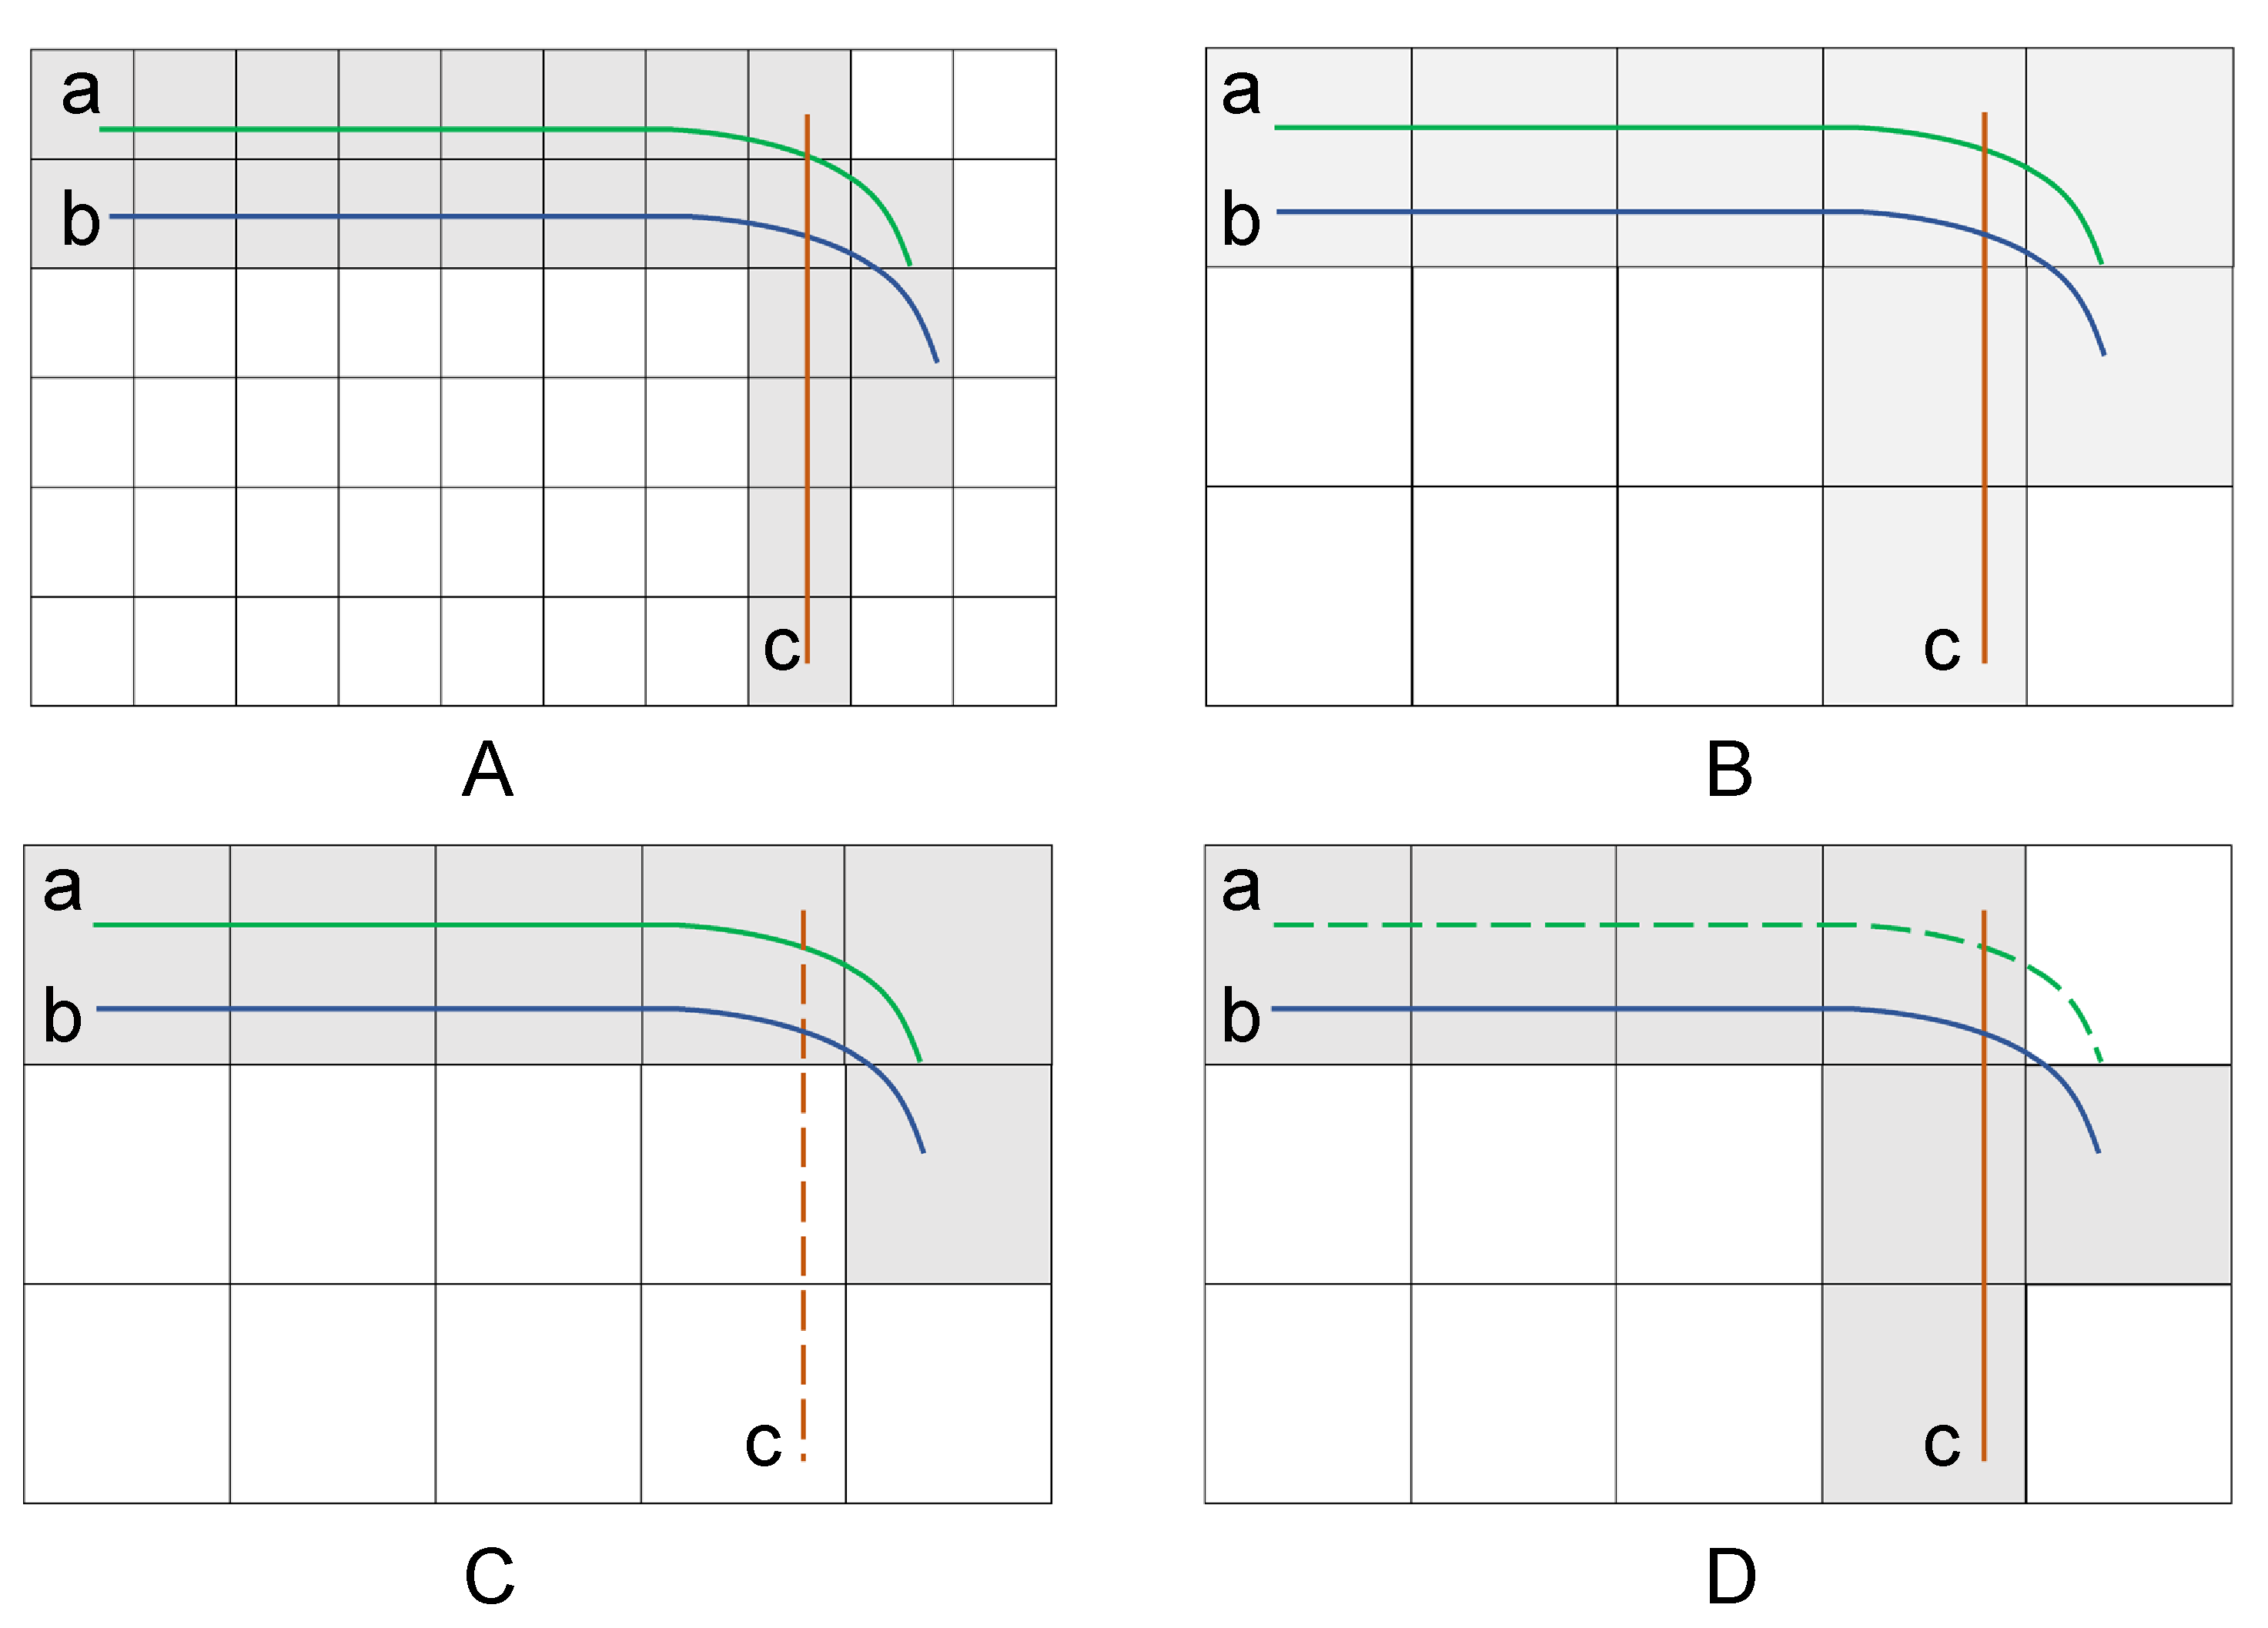
\includegraphics[width=0.4\textwidth]{pictures/problemsolveing/one_to_many.pdf}
%	\vspace{-5mm}
%	\caption{Resolution inconsistency}
%	\vspace{-5mm}
%	\label{fig:one_to_many}
%\end{figure}


% several notes for Bo, we should confirm them before submission:
% (1) rendering time,
% (2) gleaning insight from overview figures, i.e., low zoom level
% (3) delivers significantly richer information
% (4) arbitrary zooming resolutions





\section{Advance Approach: $\avats$}\label{sec:aa}
Until now, $\vats$ in Algorithm~\ref{alg:greedy} offers a visual fidelity guaranteed sampling approach for large-scale trajectory visualization problem (see Problem~\ref{prob:def}),
which returns the visual fidelity guaranteed result efficiently via the optimization techniques in Section~\ref{sec:opt}.
It means that the challenges (i) large trajectory dataset and (ii) limited rendering capability of graphics device (see Section~\ref{sec:intro}) have been addressed.
In this section, we focus on the third challenge of it, i.e.,  visual clutter.
In particular, we devise an advance approach $\avats$ to alleviate it by considering
(i) trajectory data distribution, and (ii) human perception capability.
We elaborate (i) and (ii) by the examples in Fig.~\ref{fig:delta} shortly.

\stitle{Trajectory data distribution} Considering \pt{} trajectory dataset, Fig.~\ref{fig:delta}(A) is the visualization result of $\vats$ with sampling ratio $0.5\%$.
Obviously, the real-world trajctory dataset is non-uniform distributed.
For example, the trajectories in the dense region is much more than these in the sparse region, as illustrated by the rectangles in Fig.~\ref{fig:delta}(A).

\stitle{Human perception capability} Intuitively, it is much easier for humans to distinguish the difference between sparse regions rather than dense regions in Fig.~\ref{fig:delta}(A) and (B).
The core reason is the perception capability of human beings is limited.
In particular, the visual difference of human beings will be diminished when the visualized trajectories is large enough with a given level of details,
i.e., the difference between two dense regions in Fig.~\ref{fig:delta}(A) and (B).

%instead of measuring the contribution of each trajectory w.r.t the selected trajectories in $\oR$ directly,
Taking the above two observations into consideration, the returning result of visual fidelity guaranteed sampling approach $\vats$ could be further improved by
delivering richer information at sparse regions and reducing visual clutter in dense regions.
In this section, we devise an advance approach $\avats$ (see Algorithm~\ref{alg:plus}) to achieve the above two objectives.
Specifically, we introduce perception tolerance parameter $\delta$ in $\avats$, which models human's perception capability at the most highest level of details.
In other words, suppose the pixel $(x,y)$ in canvas is covered by result set $\oR$ at the highest level,
the pixels around $(x,y)$, i.e., from $(x-\delta, y-\delta)$ to $(x+\delta, y+\delta)$, are not necessary to cover as they are in the perception tolerance of human beings.


Fortunately, we can slightly revise $\vats$ in Algorithm~\ref{alg:greedy} to incorporate the perception tolerance parameter $\delta$ in advance approach $\avats$, as shown in Algorithm~\ref{alg:plus}.
It measures the contribution of each trajectory $t_i$ w.r.t the selected trajectory set $\oR$'s augmented set $\oR^{+}$ (in Line~\ref{line:deltamax}).
The augmented set $\oR^{+}$ will be updated by the selected trajectory $tmp$ and its tolerance pixels set (in Line~\ref{line:delta}).

\vspace{-2mm}
\begin{algorithm}
    \caption{$\avats(\D,k=\alpha |\D|,\delta)$} \label{alg:plus}
    \begin{algorithmic}[1]
    \State Initialize result set $\oR \leftarrow \emptyset$
    \State Initialize augmented result set $\oR^{+} \leftarrow \emptyset$
    \While{$|\oR| < k$}
        \State $tmp \leftarrow argmax_{t_i \in \D} \oR^{+} \cup t_i$ \label{line:deltamax}
        \State $\oR \leftarrow \oR \cup \{ tmp \}$
        \State $\oR^{+} \leftarrow \oR^{+} \cup \mathsf{augment}(tmp, \delta)$\label{line:delta}
    \EndWhile
    \For{each $t$ in $\D$} \Comment{Representative encoding} \label{line:s}
        \State $tr \leftarrow argmin_{t_i \in \oR}{\mathsf{augment}(t_i, \delta) - t}$
        \State $tr.\mathsf{cnt}++$ \label{line:e}
    \EndFor
    \State Return $\oR$
    \end{algorithmic}
\end{algorithm}
\vspace{-2mm}

Interestingly, the visual clutter large trajectory visualization problem can be further reduced
by encoding representative trajectories in $\oR$ (the returning result of the advance approach $\avats$) with colors.
In particular, $\avats$ selects the trajectory which has largest uncovered pixels by taking human's perception tolerance capability into account at each iteration,
instead of only choosing the trajectory with largest uncovered pixels in $\vats$ (see Algorithm~\ref{alg:greedy}).
During its selection process, some of trajectories will not be included into the result set $\oR$ even they have more uncovered pixels w.r.t. $\oR$.
The reason is their uncovered pixels are too close to the pixels in the selected trajectories, i.e., within the tolerance area of selected pixels.
Taken Fig.~\ref{fig:zoom}(A) as example, suppose $\delta=1$ and trajectory $a$ was selected at the first iteration,
the selected trajectory in the second iteration is $c$ instead of $b$ as almost all pixels in $b$ is in the tolerance area of $a$'s.

Inherently, the $\avats$ trajectory selection process embeds the representativeness of each trajectory in the result set $\oR$.
We define the representativeness of a trajectory as the number of influenced trajectories in the dataset $\D$.
We compute the representativeness of each trajectory in $\oR$ from Line~\ref{line:s} to Line~\ref{line:e} in Algorithm~\ref{alg:plus}, then visualize them by encoding with different colors.
Fig.~\ref{fig:delta}(C) shows the visualized result of the  advance approach $\avats$ by encoding the trajectory representativeness with colors.
Obviously, the trajectories in dense region have deeper color than these in sparse regions as there many trajectories in dense region, thus the selected trajectories in the dense region are more representative.

\begin{figure}[t]
	\centering
	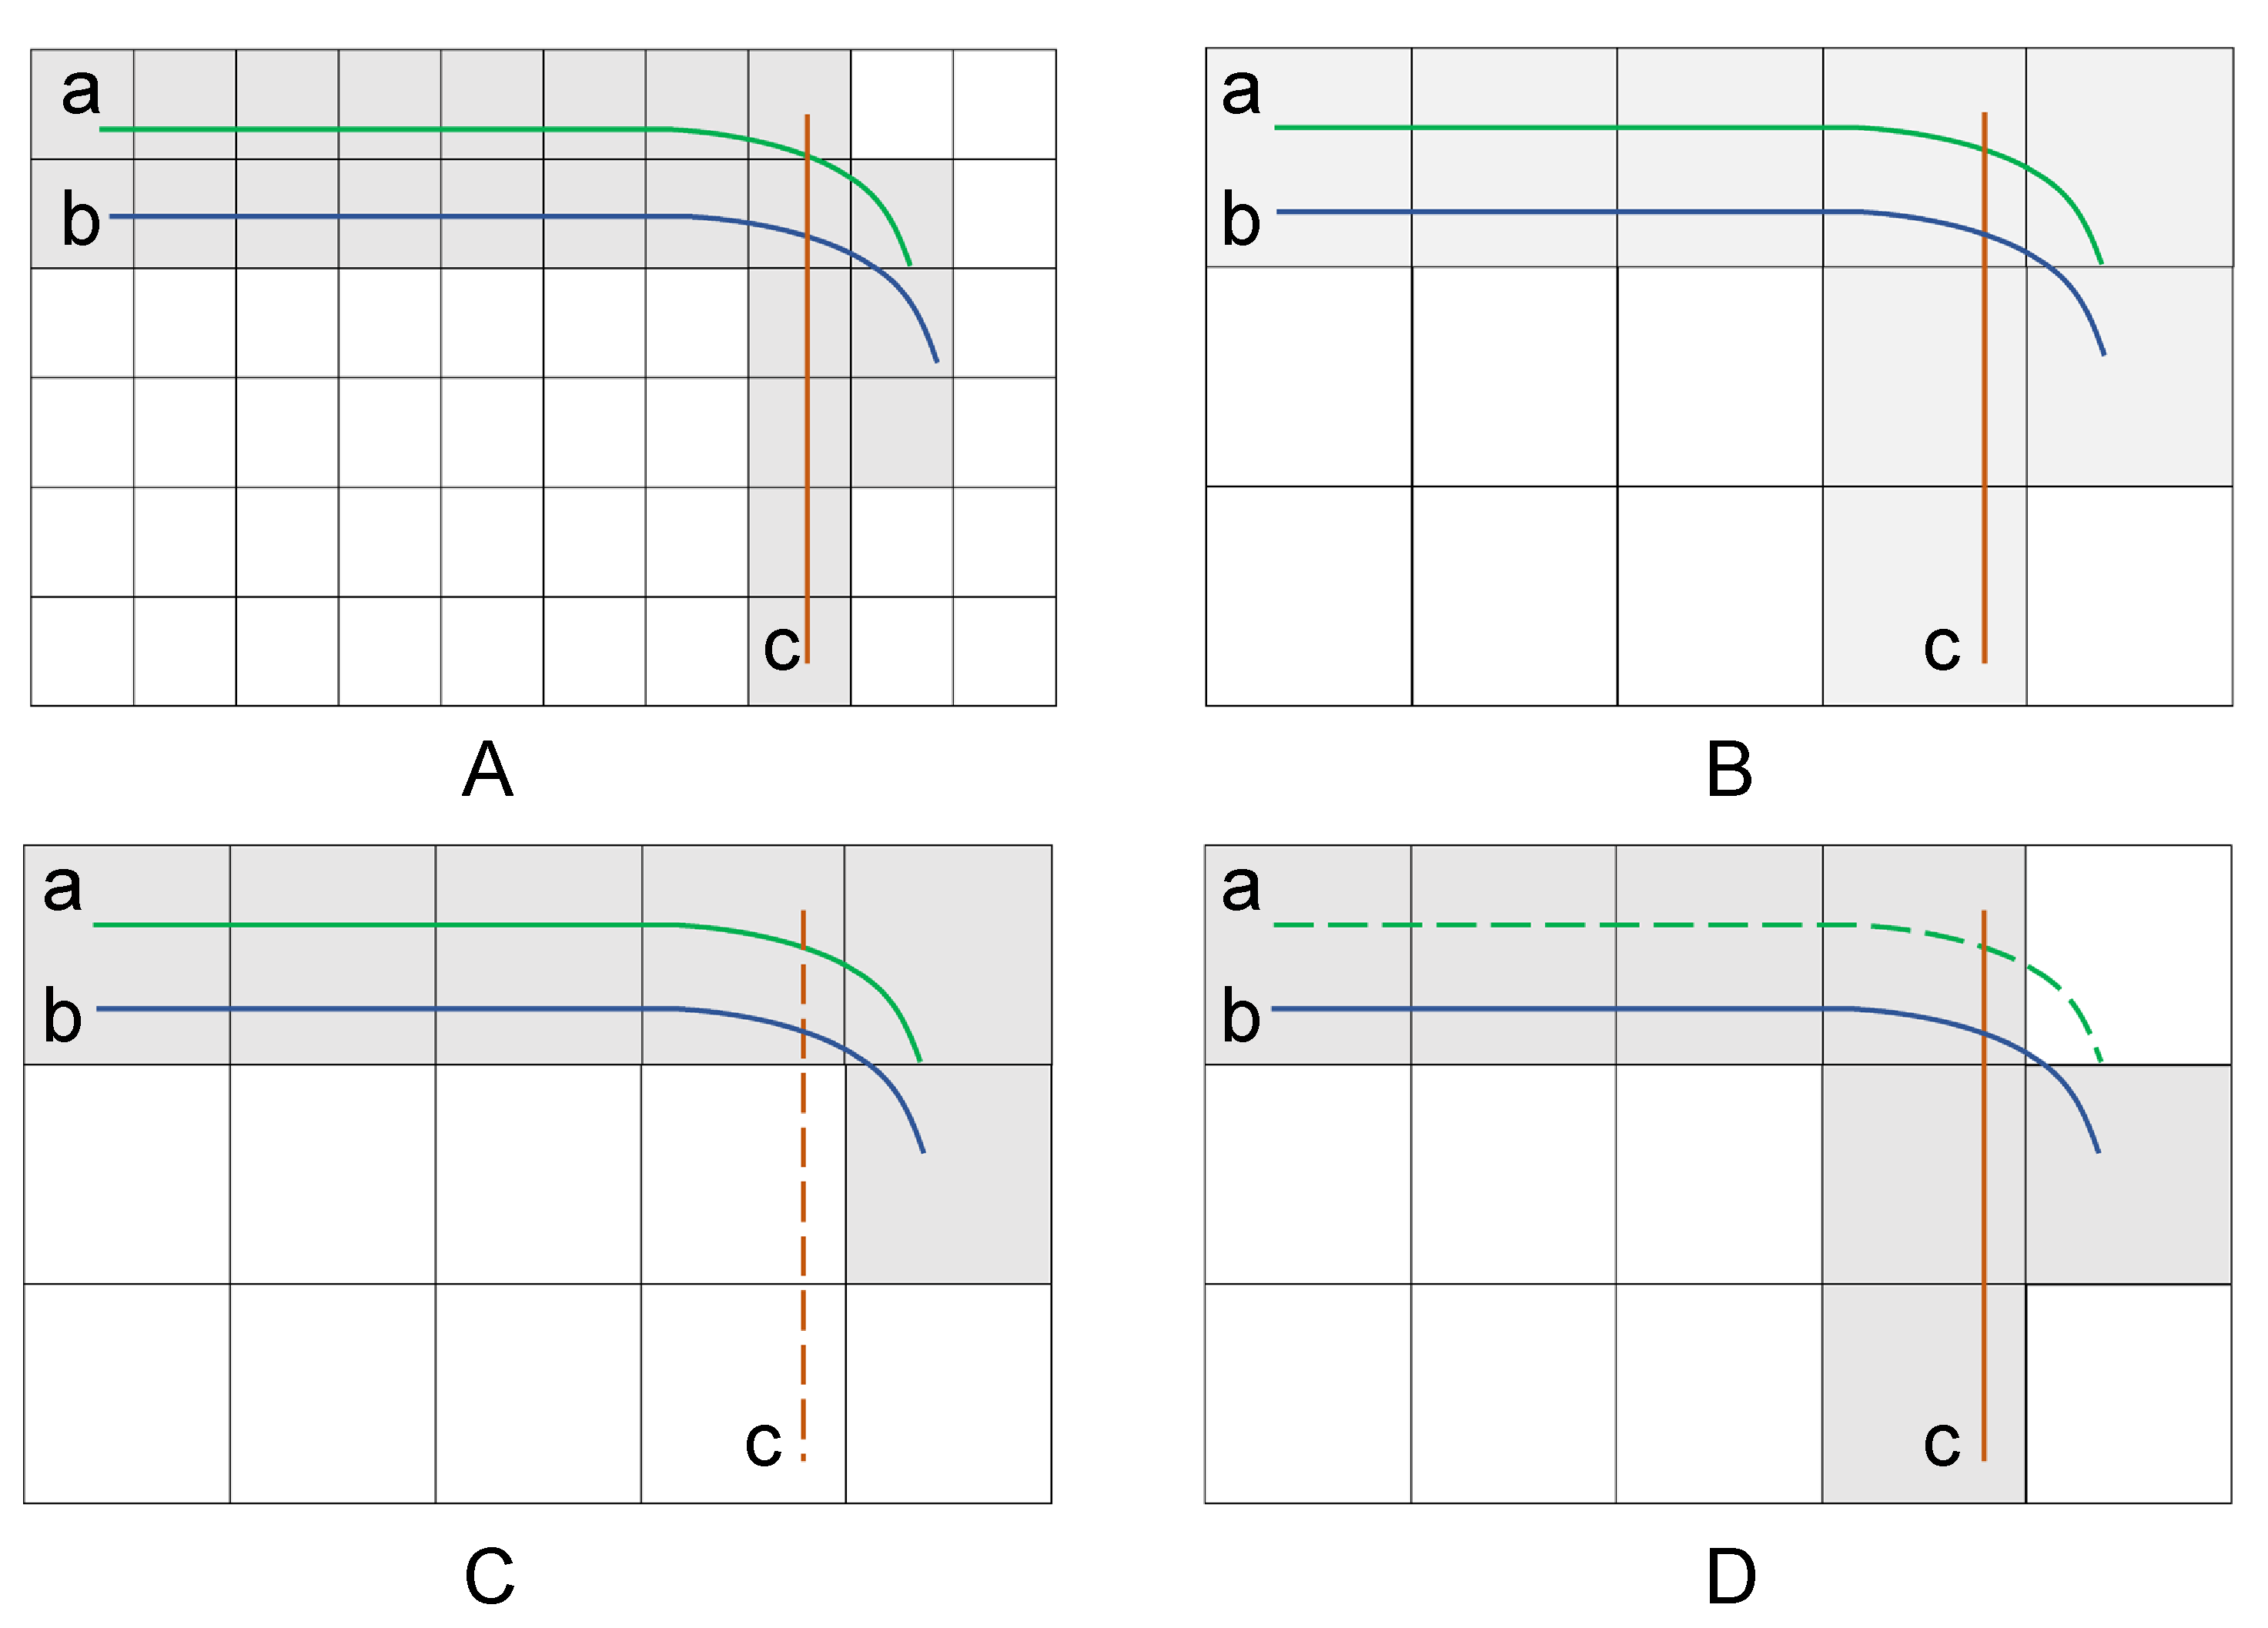
\includegraphics[width=0.4\textwidth]{pictures/problemsolveing/one_to_many.pdf}
	\vspace{-3mm}
	\caption{An illustration of $\avats$ with different zoom levels}
	\label{fig:zoom}
    \vspace{-6mm}
\end{figure}

Last but not least, it is worth to point out that our advance approach $\avats$ provides excellent visual fidelity over $\vats$ at arbitrary zooming resolutions naturally.
The key technique to achieve that is it considers the zooming resolutions inherently when introducing the perception tolerance $\delta$.
Take Fig.~\ref{fig:zoom} as an example, %Figure~\ref{fig:zoom}(A) and (B) show two different zoom-levels.
the zoom level in Fig.~\ref{fig:zoom}(A) is higher than it in Fig.~\ref{fig:zoom}(B).
As our above elaboration, our advance approach $\avats$ selects trajectory $a$ and $c$ at Fig.~\ref{fig:zoom}(A).
When it zoomed out, as shown in Fig.~\ref{fig:zoom}(b), it still captures the main sketch of the underlying dataset (as gray cells shown).




%(1) Richer Information Delivering: details aware; so Arbitrary zooming resolutions
%(2) Popularity Embedding: visual clutter



%\subsection{One-to-many strategy}~\label{sec:one_to_many}
%Since we detect the covered pixels in the highest level, two trajectories may be very close to each other but share very few pixels, which will lead to more information loss in the low zoom view as figure~\ref{fig:one_to_many}.
%We next elaborate a ``one-to-many'' strategy to further optimize the visual quality of our proposed technique.
%Recalling we use the highest zoom level to define the pixel size in the canvas.
%Thus, our visual quality guaranteed sampling algorithm is zoom-level oblivious, e.g., it guarantees the visual quality of result set $\oR$ at every zoom level.
%However, users always do not use/need the highest zoom level in visualization applications.
%For example, Google map shows city and streets at zoom level 1 and 15, respectively~\footnote{\url{https://developers.google.com/maps/documentation/}}.
%Motivated by the above observation, we devise ``one-to-many'' strategy by introducing a visual tolerance parameter $\delta$ to optimize the visual quality for users.
%Specifically, ,
%the ``one-to-many'' strategy will ignore all the pixels around $(x,y)$ within $\delta$ offset distance, i.e., all pixels from $(x-\delta, y-\delta)$ to $(x+\delta, y+\delta)$ will be skipped.
%We will demonstrate the effectiveness of the visual tolerance $\delta$ in experimental evaluations.
%
%%https://developers.google.com/maps/documentation/maps-static/dev-guide#Zoomlevels
%\begin{figure}[t]
%	\centering
%	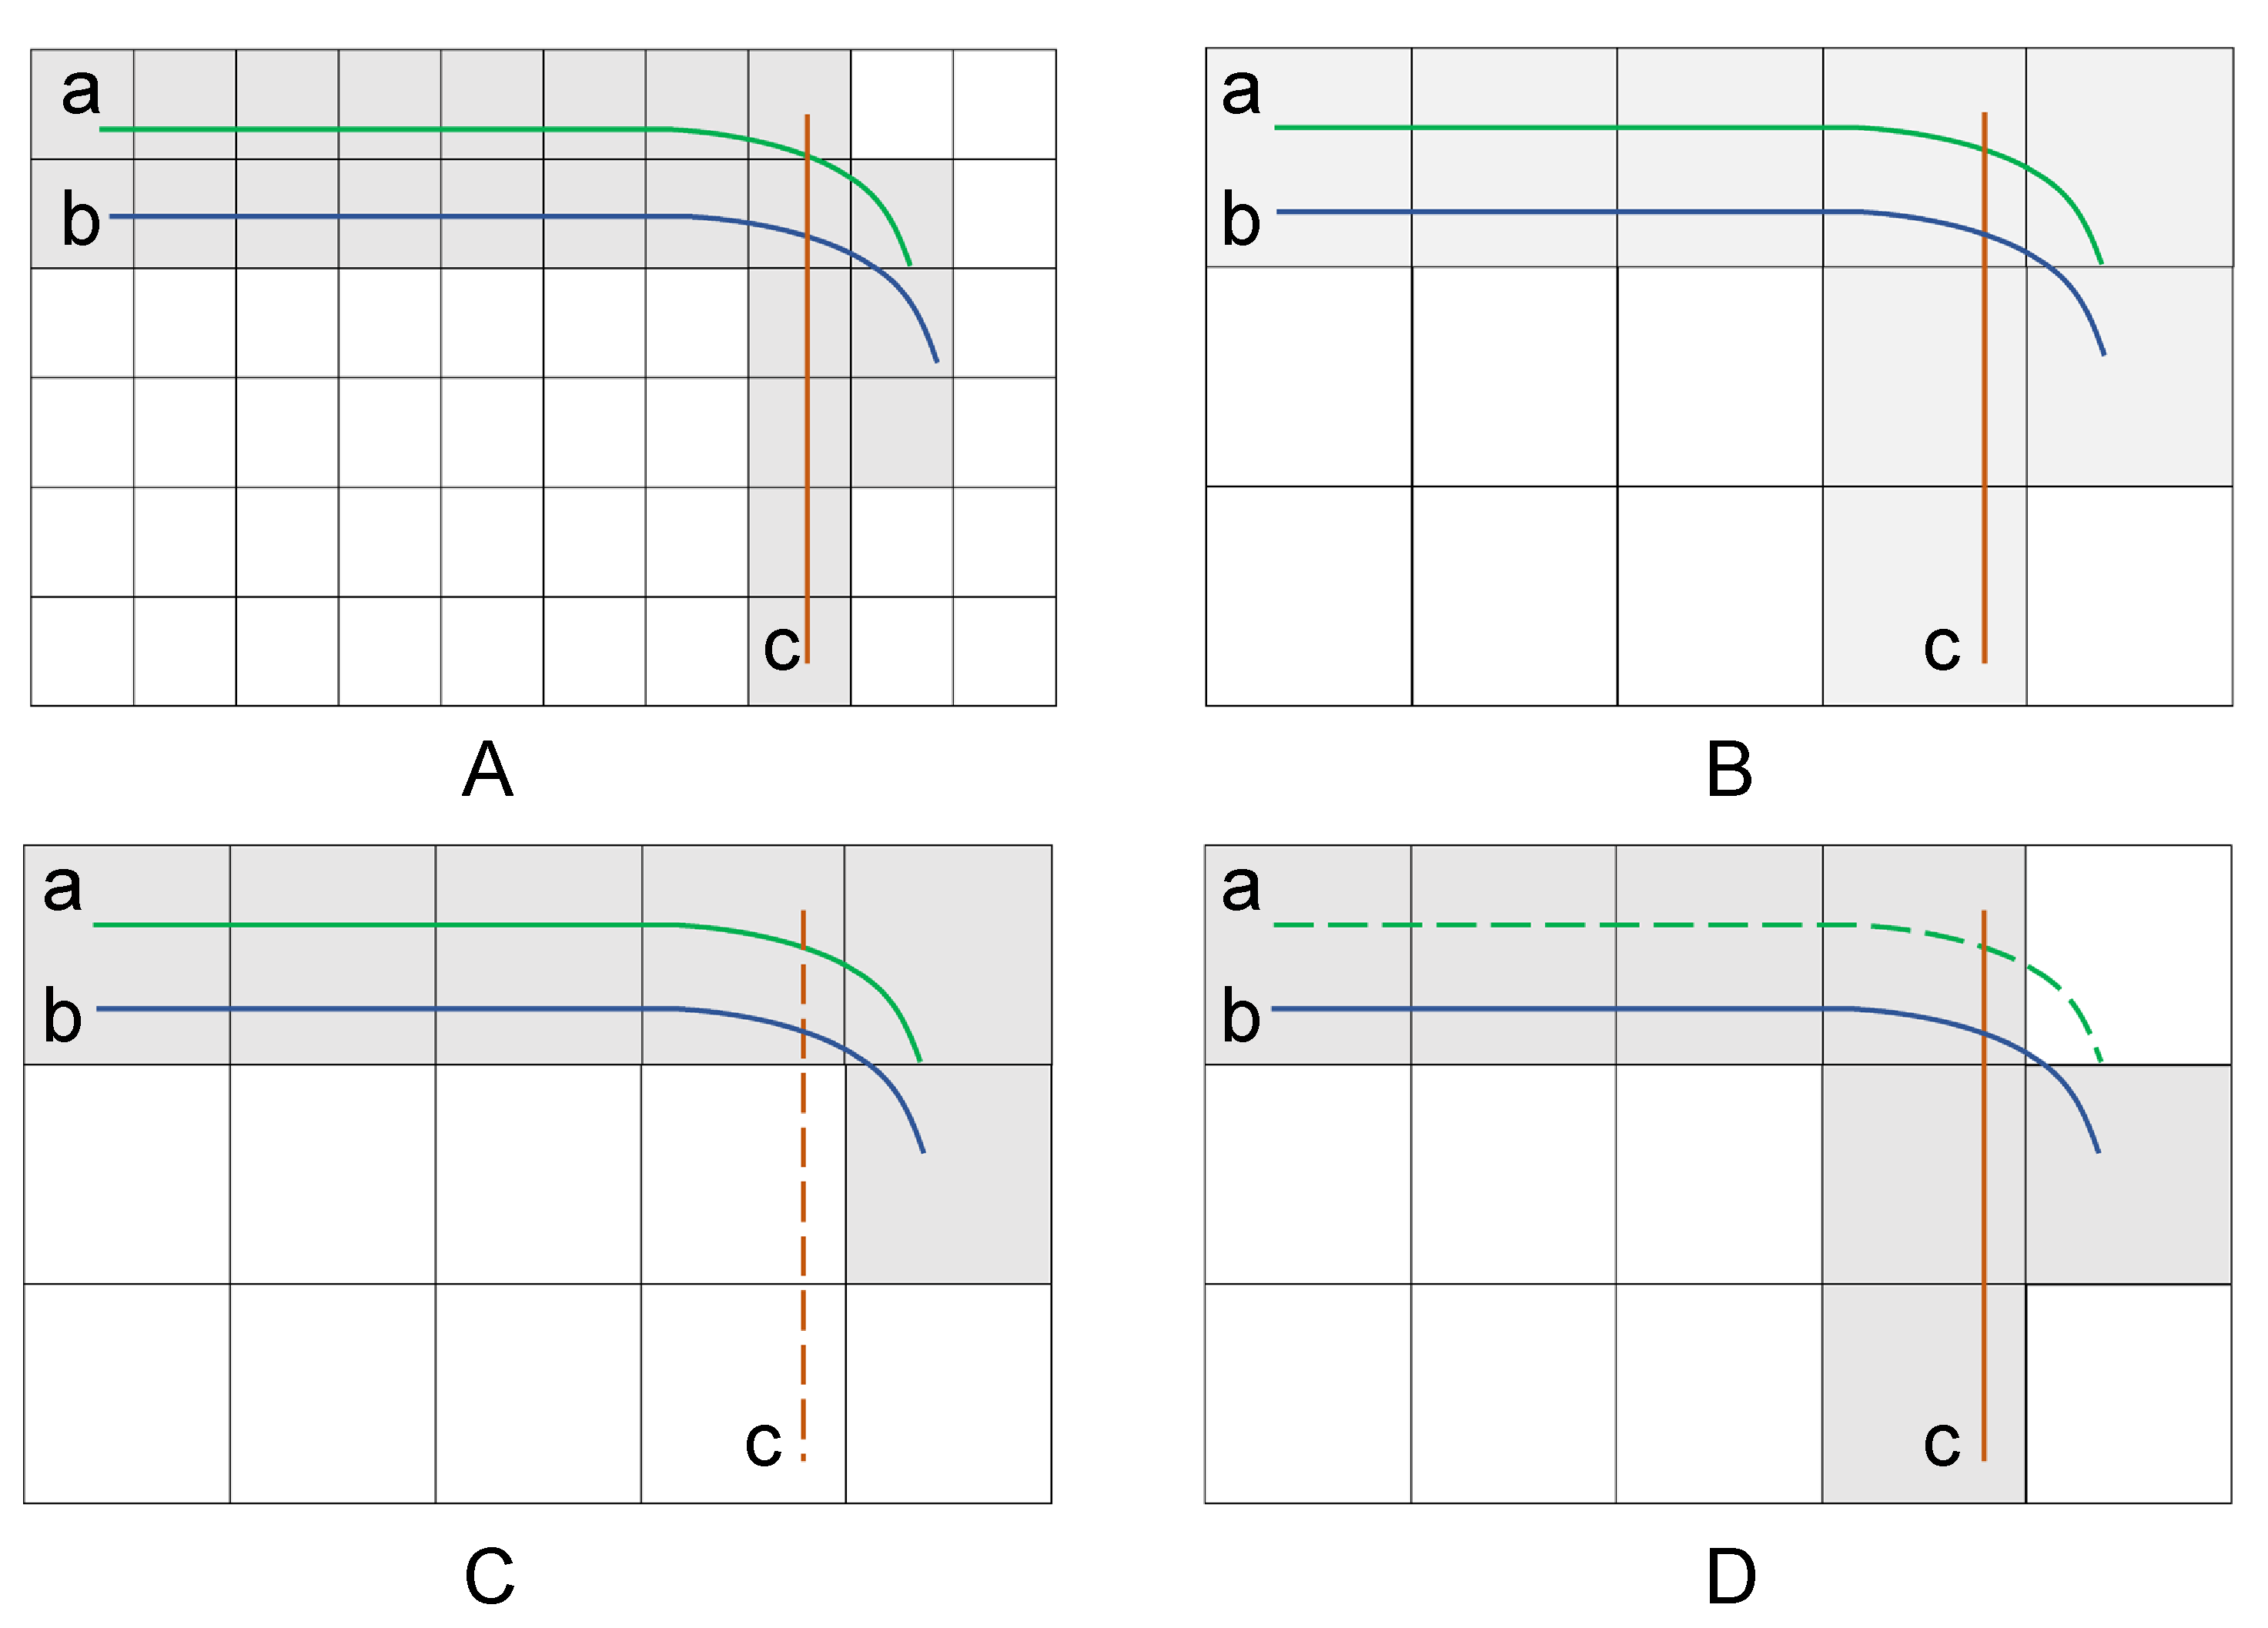
\includegraphics[width=0.4\textwidth]{pictures/problemsolveing/one_to_many.pdf}
%	\vspace{-5mm}
%	\caption{Resolution inconsistency}
%	\vspace{-5mm}
%	\label{fig:one_to_many}
%\end{figure}


%Specifically, $\avats$ incorporates a parameter $\delta$ during trajectory selection process in $\vats$ .
%In particular, we employ the parameter $\delta$ to model the end user's perception ability at the most high level of details.
%Surprisingly, our advance approach $\avats$ not only provides better visualization result when comparing with $\vats$ with the same sampling rate
%(e.g., Figure~\ref{fig:delta}(a) and (b) are the returning result of $\vats$ and $\avats$ respectively),
%but also embeds the popularity of selected trajectories by encoding the rest trajectories in the dataset in them,
%e.g., Figure~\ref{fig:delta}(c) is the visual result of $\avats$ with color encoded popularity.


